%%%%%%%%%%%%%%%%%%%%%%%%%%%%%%%%%%%%%%%%%%%%%%%%%%%%%%%%%%%%%%%%%%%%%%%%%%%%%%%%
%2345678901234567890123456789012345678901234567890123456789012345678901234567890
%        1         2         3         4         5         6         7         8

\documentclass[letterpaper, 12 pt, conference]{ieeeconf}  % Comment this line out
                                                          % if you need a4paper
%\documentclass[a4paper, 12pt, conference]{ieeeconf}      % Use this line for a4
                                                          % paper

\IEEEoverridecommandlockouts                              % This command is only
                                                          % needed if you want to
                                                          % use the \thanks command
\overrideIEEEmargins
% See the \addtolength command later in the file to balance the column lengths
% on the last page of the document

\usepackage{hyperref}
\usepackage[utf8]{inputenc}
\usepackage{enumerate}
\usepackage{natbib}
\usepackage{graphicx}
\usepackage[spanish]{babel}
\hypersetup{
    colorlinks=true,
    linkcolor=blue,
    filecolor=magenta,      
    urlcolor=cyan,
}

% The following packages can be found on http:\\www.ctan.org
%\usepackage{graphics} % for pdf, bitmapped graphics files
%\usepackage{epsfig} % for postscript graphics files
%\usepackage{mathptmx} % assumes new font selection scheme installed
%\usepackage{times} % assumes new font selection scheme installed
%\usepackage{amsmath} % assumes amsmath package installed
%\usepackage{amssymb}  % assumes amsmath package installed

\title{\LARGE \bf
Práctica 1: redes resistivas
}

%\author{ \parbox{3 in}{\centering Narshion Ngao*
%         \thanks{*Use the $\backslash$thanks command to put information here}\\
%         Msc. Computer Systems - 2018\\
%         Jomo Kenyatta University of Agriculture \& Technology \\
%       
%}}

\author{Universidad de San Carlos de Guatemala \\% <-this % stops a space
Escuela de Ciencias Físicas y Matemáticas\\
Laboratorio de Circuitos\\
Segundo Semestre 2019
}


\begin{document}



\maketitle
\thispagestyle{empty}
\pagestyle{empty}

\section{Objetivos}
\begin{itemize}
    \item General: Ejercitar los conceptos básicos de redes de resistencias y mediciones con multímetro vistos en lecciones anteriores.
    \item Específicos:
    \begin{enumerate}
    \item Practicar el uso correcto del multímetro para medición de voltaje, corriente y resistencia.
    \item Confirmar la exactitud de la Ley de Ohm para el cálculo de magnitudes en dispositivos óhmicos vs los valores prácticos.
    \item Comprobar empíricamente la equivalencia de de magnitudes en una red escalera.
\end{enumerate}
\end{itemize}


\section{Materiales}
\begin{enumerate}
    \item 1 mina de grafito 6B o superior (puede ser lápiz).
    \item 1 regla.
    \item 1 hoja de papel bond.
    \item 1 multímetro.
    \item 10 resistencias de cualquier valor 1/4W.
    \item 1 potenciómetro de 1K ohm.
    \item Alambres para protoboard de cualquier tipo (y pinzas para cortarlo, si es necesario).
    \item 1 fuente.
    \item 1 protoboard.
    \item Opcional: computadora con software para generación de graficas.
\end{enumerate}
\pagebreak

\section{Diagramas}

\begin{figure}[h!]
    \centering
    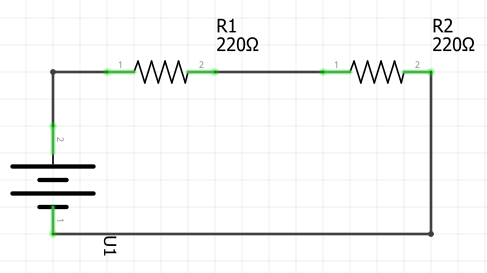
\includegraphics[scale=0.7]{C1.png}
    \caption{Esquema de circuito inicial.}
\end{figure}

\begin{figure}[h!]
    \centering
    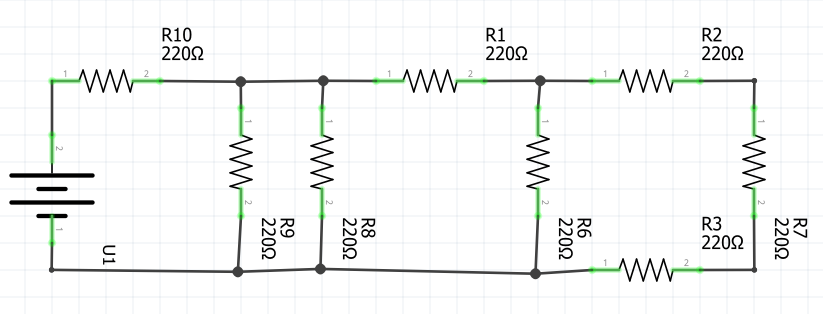
\includegraphics[scale=0.5]{C2.png}
    \caption{Esquema red escalera.}
\end{figure}


\section{Procedimiento y reporte de resultados}
Seguir todos los pasos que a continuación se enlistan respondiendo en una hoja adicional lo que sea requerido de forma ORDENADA y CLARA.

\begin{enumerate}
    \item Dibujar en la hoja de papel bond cuatro rectángulos de 15 cm de largo y anchos 0.2, 0.7, 1.2 y 1.7 cm. 
    \item Rellenar los rectángulos con el grafito cuidando de no romper el papel ni dejar espacios en blanco.
    \item Marcar para cada rectángulo espacios de 3 cm de separación en toda la longitud.
    \item Con un multímetro en la opción de óhmetro, medir la resistencia de cada rectángulo con el fin de llenar una tabla similar a la siguiente para cada rectángulo:
    
\begin{table}[h!]
 \centering
\begin{tabular}{|c|l|l|l|}
\hline
\multicolumn{4}{|c|}{Grosor 1: 0.2 cm}                                                                                                 \\ \hline
\multicolumn{1}{|l|}{\textbf{No.}} & \textbf{R$\pm \Delta$R} & \textbf{L$\pm \Delta$L} & \multicolumn{1}{c|}{\textbf{Longitud/Grosor$\pm \Delta$}} \\ \hline
1                                  &                         &                         &                                               \\ \hline
2                                  &                         &                         &                                               \\ \hline
3                                  &                         &                         &                                               \\ \hline
4                                  &                         &                         &                                               \\ \hline
5                                  &                         &                         &                                               \\ \hline
\end{tabular}
\end{table}

    \item Reordenar los datos obtenidos en tablas correspondientes a las magnitudes medidas para cada longitud en todos los rectángulos.

\begin{table}[h!]
\centering
\begin{tabular}{|c|l|l|}
\hline
\multicolumn{3}{|c|}{Longitud: 3 cm}                                                                                 \\ \hline
\multicolumn{1}{|l|}{\textbf{No.}} & \textbf{R$\pm \Delta$R} & \textbf{G$\pm \Delta$G} \\ \hline
1                                  &                         & 0.2 cm                                                \\ \hline
2                                  &                         & 0.7 cm                                                \\ \hline
3                                  &                         & 1.2 cm                                                \\ \hline
4                                  &                         & 1.7 cm                                                \\ \hline
\end{tabular}
\end{table}

    \item Realizar gráficas R vs L para cada rectángulo (4 en total).
    \item Realizar gráficas R vs G (5 en total).
    \item Anotar tres conclusiones parciales de los resultados obtenidos hasta el momento.
    \item Realizar gráficas R vs L/G para cada rectángulo (4 en total).
    \item Comparar los resultados visuales obtenidos con la ecuación de la ressitencia en función de su geometría. ¿Las magnitudes medidas obedecen a la ecuación? Explicar detalladamente.
    \item Armar en un protoboard el divisor de voltaje de la Figura 1 con dos resistencias fijas (idealmente del mismo valor).

\begin{figure}[h!]
    \centering
    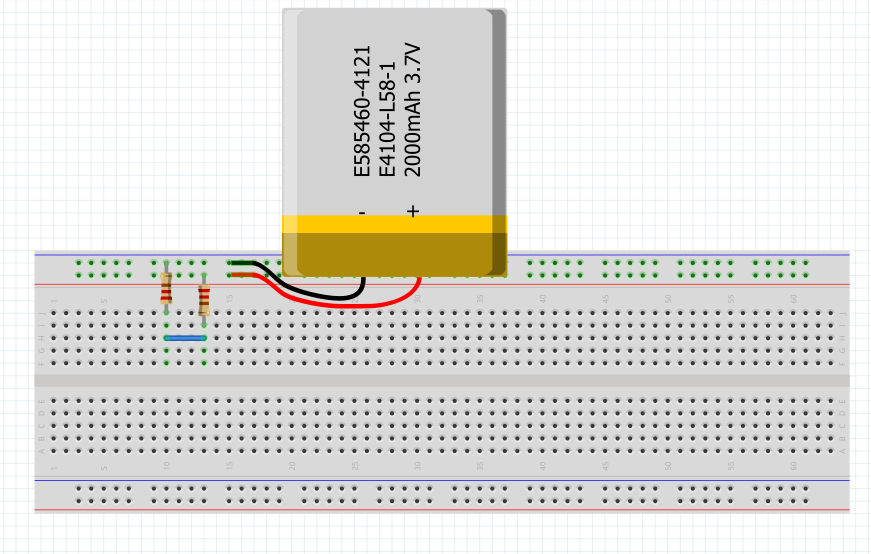
\includegraphics[scale=0.4]{B1.png}
    \caption{Circuito de Figura 1 en protoboard.}
\end{figure}
    \item Calcular por Ley de Ohm la magnitud de la corriente en la malla y el voltaje en R2 (con valores ideales).
    \item Con un multímetro, medir los valores reales del inciso anterior y realizar un pequeño diagrama de incertezas para comparar. ¿Los valores coincidieron?
    \item Con ayuda de un potenciómetro, variar el valor de R2. Anotar en una tabla 5 variaciones de resistencia vs voltaje.¿Cómo se comporta el voltaje en el divisor según la resistencia aumenta y disminuye?
    \item Armar en protoboard la red escalera de la Figura 2.
    
\begin{figure}[h!]
    \centering
    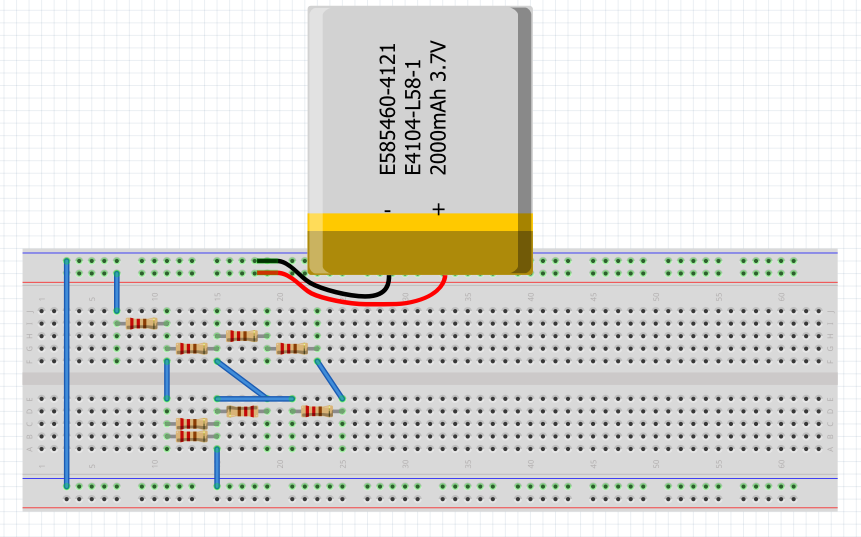
\includegraphics[scale=0.4]{B2.png}
    \caption{Circuito de Figura 2 en protoboard.}
\end{figure}
    
    \item Reducir las resistencias en serie y paralelo para obtener una equivalente en serie con la fuente. Calcular la corriente teórica total que la fuente entrega al circuito.
    \item Medir con un multímetro en función de amperímetro la corriente en R10. ¿Coincidió con el valor calculado en el inciso anterior? ¿Por qué?
    \item Medir el voltaje en R9 y el de R8. 
    \item Medir el voltaje de R2, R7 y R3 juntas. ¿Qué puede concluirse de los valores obtenidos en los últimos dos incisos?
    \item Medir el voltaje solamente en R7. ¿Fue el mismo que en R9? ¿Por qué?
    \item Escribir las conclusiones generales de la práctica.
\end{enumerate}
\addtolength{\textheight}{-12cm}   % This command serves to balance the column lengths
                                  % on the last page of the document manually. It shortens
                                  % the textheight of the last page by a suitable amount.
                                  % This command does not take effect until the next page
                                  % so it should come on the page before the last. Make
                                  % sure that you do not shorten the textheight too much.

\end{document}